\documentclass[1p]{elsarticle_modified}
%\bibliographystyle{elsarticle-num}

%\usepackage[colorlinks]{hyperref}
%\usepackage{abbrmath_seonhwa} %\Abb, \Ascr, \Acal ,\Abf, \Afrak
\usepackage{amsfonts}
\usepackage{amssymb}
\usepackage{amsmath}
\usepackage{amsthm}
\usepackage{scalefnt}
\usepackage{amsbsy}
\usepackage{kotex}
\usepackage{caption}
\usepackage{subfig}
\usepackage{color}
\usepackage{graphicx}
\usepackage{xcolor} %% white, black, red, green, blue, cyan, magenta, yellow
\usepackage{float}
\usepackage{setspace}
\usepackage{hyperref}

\usepackage{tikz}
\usetikzlibrary{arrows}

\usepackage{multirow}
\usepackage{array} % fixed length table
\usepackage{hhline}

%%%%%%%%%%%%%%%%%%%%%
\makeatletter
\renewcommand*\env@matrix[1][\arraystretch]{%
	\edef\arraystretch{#1}%
	\hskip -\arraycolsep
	\let\@ifnextchar\new@ifnextchar
	\array{*\c@MaxMatrixCols c}}
\makeatother %https://tex.stackexchange.com/questions/14071/how-can-i-increase-the-line-spacing-in-a-matrix
%%%%%%%%%%%%%%%

\usepackage[normalem]{ulem}

\newcommand{\msout}[1]{\ifmmode\text{\sout{\ensuremath{#1}}}\else\sout{#1}\fi}
%SOURCE: \msout is \stkout macro in https://tex.stackexchange.com/questions/20609/strikeout-in-math-mode

\newcommand{\cancel}[1]{
	\ifmmode
	{\color{red}\msout{#1}}
	\else
	{\color{red}\sout{#1}}
	\fi
}

\newcommand{\add}[1]{
	{\color{blue}\uwave{#1}}
}

\newcommand{\replace}[2]{
	\ifmmode
	{\color{red}\msout{#1}}{\color{blue}\uwave{#2}}
	\else
	{\color{red}\sout{#1}}{\color{blue}\uwave{#2}}
	\fi
}

\newcommand{\Sol}{\mathcal{S}} %segment
\newcommand{\D}{D} %diagram
\newcommand{\A}{\mathcal{A}} %arc


%%%%%%%%%%%%%%%%%%%%%%%%%%%%%5 test

\def\sl{\operatorname{\textup{SL}}(2,\Cbb)}
\def\psl{\operatorname{\textup{PSL}}(2,\Cbb)}
\def\quan{\mkern 1mu \triangleright \mkern 1mu}

\theoremstyle{definition}
\newtheorem{thm}{Theorem}[section]
\newtheorem{prop}[thm]{Proposition}
\newtheorem{lem}[thm]{Lemma}
\newtheorem{ques}[thm]{Question}
\newtheorem{cor}[thm]{Corollary}
\newtheorem{defn}[thm]{Definition}
\newtheorem{exam}[thm]{Example}
\newtheorem{rmk}[thm]{Remark}
\newtheorem{alg}[thm]{Algorithm}

\newcommand{\I}{\sqrt{-1}}
\begin{document}

%\begin{frontmatter}
%
%\title{Boundary parabolic representations of knots up to 8 crossings}
%
%%% Group authors per affiliation:
%\author{Yunhi Cho} 
%\address{Department of Mathematics, University of Seoul, Seoul, Korea}
%\ead{yhcho@uos.ac.kr}
%
%
%\author{Seonhwa Kim} %\fnref{s_kim}}
%\address{Center for Geometry and Physics, Institute for Basic Science, Pohang, 37673, Korea}
%\ead{ryeona17@ibs.re.kr}
%
%\author{Hyuk Kim}
%\address{Department of Mathematical Sciences, Seoul National University, Seoul 08826, Korea}
%\ead{hyukkim@snu.ac.kr}
%
%\author{Seokbeom Yoon}
%\address{Department of Mathematical Sciences, Seoul National University, Seoul, 08826,  Korea}
%\ead{sbyoon15@snu.ac.kr}
%
%\begin{abstract}
%We find all boundary parabolic representation of knots up to 8 crossings.
%
%\end{abstract}
%\begin{keyword}
%    \MSC[2010] 57M25 
%\end{keyword}
%
%\end{frontmatter}

%\linenumbers
%\tableofcontents
%
\newcommand\colored[1]{\textcolor{white}{\rule[-0.35ex]{0.8em}{1.4ex}}\kern-0.8em\color{red} #1}%
%\newcommand\colored[1]{\textcolor{white}{ #1}\kern-2.17ex	\textcolor{white}{ #1}\kern-1.81ex	\textcolor{white}{ #1}\kern-2.15ex\color{red}#1	}

{\Large $\underline{12a_{0266}~(K12a_{0266})}$}

\setlength{\tabcolsep}{10pt}
\renewcommand{\arraystretch}{1.6}
\vspace{1cm}\begin{tabular}{m{100pt}>{\centering\arraybackslash}m{274pt}}
\multirow{5}{120pt}{
	\centering
	\includegraphics[width=112pt]{../../../GIT/diagram.site/Diagrams/png/1067_12a_0266.png}\\
\ \ \ A knot diagram\footnotemark}&
\allowdisplaybreaks
\textbf{Linearized knot diagam} \\
\cline{2-2}
 &
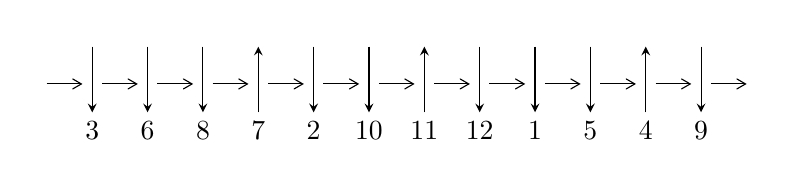
\begin{tikzpicture}[x=20pt, y=17pt]
	% nodes
	\node (C0) at (0, 0) {};
	\node (C1) at (1, 0) {};
	\node (C1U) at (1, +1) {};
	\node (C1D) at (1, -1) {3};

	\node (C2) at (2, 0) {};
	\node (C2U) at (2, +1) {};
	\node (C2D) at (2, -1) {6};

	\node (C3) at (3, 0) {};
	\node (C3U) at (3, +1) {};
	\node (C3D) at (3, -1) {8};

	\node (C4) at (4, 0) {};
	\node (C4U) at (4, +1) {};
	\node (C4D) at (4, -1) {7};

	\node (C5) at (5, 0) {};
	\node (C5U) at (5, +1) {};
	\node (C5D) at (5, -1) {2};

	\node (C6) at (6, 0) {};
	\node (C6U) at (6, +1) {};
	\node (C6D) at (6, -1) {10};

	\node (C7) at (7, 0) {};
	\node (C7U) at (7, +1) {};
	\node (C7D) at (7, -1) {11};

	\node (C8) at (8, 0) {};
	\node (C8U) at (8, +1) {};
	\node (C8D) at (8, -1) {12};

	\node (C9) at (9, 0) {};
	\node (C9U) at (9, +1) {};
	\node (C9D) at (9, -1) {1};

	\node (C10) at (10, 0) {};
	\node (C10U) at (10, +1) {};
	\node (C10D) at (10, -1) {5};

	\node (C11) at (11, 0) {};
	\node (C11U) at (11, +1) {};
	\node (C11D) at (11, -1) {4};

	\node (C12) at (12, 0) {};
	\node (C12U) at (12, +1) {};
	\node (C12D) at (12, -1) {9};
	\node (C13) at (13, 0) {};

	% arrows
	\draw[->,>={angle 60}]
	(C0) edge (C1) (C1) edge (C2) (C2) edge (C3) (C3) edge (C4) (C4) edge (C5) (C5) edge (C6) (C6) edge (C7) (C7) edge (C8) (C8) edge (C9) (C9) edge (C10) (C10) edge (C11) (C11) edge (C12) (C12) edge (C13) ;	\draw[->,>=stealth]
	(C1U) edge (C1D) (C2U) edge (C2D) (C3U) edge (C3D) (C4D) edge (C4U) (C5U) edge (C5D) (C6U) edge (C6D) (C7D) edge (C7U) (C8U) edge (C8D) (C9U) edge (C9D) (C10U) edge (C10D) (C11D) edge (C11U) (C12U) edge (C12D) ;
	\end{tikzpicture} \\
\hhline{~~} \\& 
\textbf{Solving Sequence} \\ \cline{2-2} 
 &
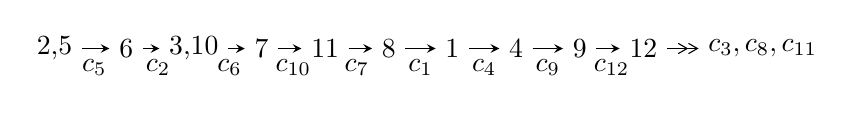
\begin{tikzpicture}[x=23pt, y=7pt]
	% node
	\node (A0) at (-1/8, 0) {2,5};
	\node (A1) at (1, 0) {6};
	\node (A2) at (33/16, 0) {3,10};
	\node (A3) at (25/8, 0) {7};
	\node (A4) at (33/8, 0) {11};
	\node (A5) at (41/8, 0) {8};
	\node (A6) at (49/8, 0) {1};
	\node (A7) at (57/8, 0) {4};
	\node (A8) at (65/8, 0) {9};
	\node (A9) at (73/8, 0) {12};
	\node (C1) at (1/2, -1) {$c_{5}$};
	\node (C2) at (3/2, -1) {$c_{2}$};
	\node (C3) at (21/8, -1) {$c_{6}$};
	\node (C4) at (29/8, -1) {$c_{10}$};
	\node (C5) at (37/8, -1) {$c_{7}$};
	\node (C6) at (45/8, -1) {$c_{1}$};
	\node (C7) at (53/8, -1) {$c_{4}$};
	\node (C8) at (61/8, -1) {$c_{9}$};
	\node (C9) at (69/8, -1) {$c_{12}$};
	\node (A10) at (11, 0) {$c_{3},c_{8},c_{11}$};

	% edge
	\draw[->,>=stealth]	
	(A0) edge (A1) (A1) edge (A2) (A2) edge (A3) (A3) edge (A4) (A4) edge (A5) (A5) edge (A6) (A6) edge (A7) (A7) edge (A8) (A8) edge (A9) ;
	\draw[->>,>={angle 60}]	
	(A9) edge (A10);
\end{tikzpicture} \\ 

\end{tabular} \\

\footnotetext{
The image of knot diagram is generated by the software ``\textbf{Draw programme}" developed by Andrew Bartholomew(\url{http://www.layer8.co.uk/maths/draw/index.htm\#Running-draw}), where we modified some parts for our purpose(\url{https://github.com/CATsTAILs/LinksPainter}).
}\phantom \\ \newline 
\centering \textbf{Ideals for irreducible components\footnotemark of $X_{\text{par}}$} 
 
\begin{align*}
I^u_{1}&=\langle 
-5.65100\times10^{376} u^{138}-1.59780\times10^{377} u^{137}+\cdots+1.07658\times10^{378} b-5.53322\times10^{378},\\
\phantom{I^u_{1}}&\phantom{= \langle  }1.04283\times10^{379} u^{138}+2.43820\times10^{379} u^{137}+\cdots+5.92116\times10^{379} a-1.92434\times10^{381},\\
\phantom{I^u_{1}}&\phantom{= \langle  }u^{139}+4 u^{138}+\cdots+472 u-55\rangle \\
I^u_{2}&=\langle 
10 u^{18}-3 u^{17}+\cdots+b-10,\;9 u^{18}- u^{17}+\cdots+a-7,\;u^{19}- u^{18}+\cdots-3 u+1\rangle \\
I^u_{3}&=\langle 
- u^2 a+a u- u^2+b+u-1,\;u^2 a+a^2-3 a u+3 u^2+2 a-3 u+2,\;u^3- u^2+1\rangle \\
I^u_{4}&=\langle 
-3 a^3+2 a^2+31 b-8 a+6,\;a^4- a^3-4 a^2+4 a+11,\;u+1\rangle \\
\\
\end{align*}
\raggedright * 4 irreducible components of $\dim_{\mathbb{C}}=0$, with total 168 representations.\\
\footnotetext{All coefficients of polynomials are rational numbers. But the coefficients are sometimes approximated in decimal forms when there is not enough margin.}
\newpage
\renewcommand{\arraystretch}{1}
\centering \section*{I. $I^u_{1}= \langle -5.65\times10^{376} u^{138}-1.60\times10^{377} u^{137}+\cdots+1.08\times10^{378} b-5.53\times10^{378},\;1.04\times10^{379} u^{138}+2.44\times10^{379} u^{137}+\cdots+5.92\times10^{379} a-1.92\times10^{381},\;u^{139}+4 u^{138}+\cdots+472 u-55 \rangle$}
\flushleft \textbf{(i) Arc colorings}\\
\begin{tabular}{m{7pt} m{180pt} m{7pt} m{180pt} }
\flushright $a_{2}=$&$\begin{pmatrix}0\\u\end{pmatrix}$ \\
\flushright $a_{5}=$&$\begin{pmatrix}1\\0\end{pmatrix}$ \\
\flushright $a_{6}=$&$\begin{pmatrix}1\\u^2\end{pmatrix}$ \\
\flushright $a_{3}=$&$\begin{pmatrix}- u\\- u^3+u\end{pmatrix}$ \\
\flushright $a_{10}=$&$\begin{pmatrix}-0.176119 u^{138}-0.411777 u^{137}+\cdots-182.170 u+32.4994\\0.0524905 u^{138}+0.148415 u^{137}+\cdots-54.4052 u+5.13965\end{pmatrix}$ \\
\flushright $a_{7}=$&$\begin{pmatrix}-0.00182425 u^{138}-0.00973214 u^{137}+\cdots-175.493 u+13.5208\\0.144407 u^{138}+0.352288 u^{137}+\cdots+58.8870 u-6.47093\end{pmatrix}$ \\
\flushright $a_{11}=$&$\begin{pmatrix}-0.228609 u^{138}-0.560192 u^{137}+\cdots-127.765 u+27.3597\\0.0524905 u^{138}+0.148415 u^{137}+\cdots-54.4052 u+5.13965\end{pmatrix}$ \\
\flushright $a_{8}=$&$\begin{pmatrix}-0.586546 u^{138}-1.77386 u^{137}+\cdots-408.709 u+48.7522\\0.508633 u^{138}+1.39800 u^{137}+\cdots+106.194 u-12.7124\end{pmatrix}$ \\
\flushright $a_{1}=$&$\begin{pmatrix}u^3\\u^5- u^3+u\end{pmatrix}$ \\
\flushright $a_{4}=$&$\begin{pmatrix}0.125067 u^{138}+0.930157 u^{137}+\cdots-129.743 u+15.4604\\-0.100367 u^{138}-0.428049 u^{137}+\cdots-80.1730 u+9.18097\end{pmatrix}$ \\
\flushright $a_{9}=$&$\begin{pmatrix}-0.226178 u^{138}-0.541512 u^{137}+\cdots-136.597 u+27.7184\\0.0388748 u^{138}+0.0924747 u^{137}+\cdots-31.6327 u+2.65267\end{pmatrix}$ \\
\flushright $a_{12}=$&$\begin{pmatrix}-0.607158 u^{138}-2.10441 u^{137}+\cdots-159.069 u+30.0427\\0.206637 u^{138}+0.507832 u^{137}+\cdots+37.1120 u-5.50176\end{pmatrix}$\\&\end{tabular}
\flushleft \textbf{(ii) Obstruction class $= -1$}\\~\\
\flushleft \textbf{(iii) Cusp Shapes $= 0.0201009 u^{138}-0.638391 u^{137}+\cdots-384.484 u+31.1094$}\\~\\
\newpage\renewcommand{\arraystretch}{1}
\flushleft \textbf{(iv) u-Polynomials at the component}\newline \\
\begin{tabular}{m{50pt}|m{274pt}}
Crossings & \hspace{64pt}u-Polynomials at each crossing \\
\hline $$\begin{aligned}c_{1}\end{aligned}$$&$\begin{aligned}
&u^{139}+62 u^{138}+\cdots+388114 u+3025
\end{aligned}$\\
\hline $$\begin{aligned}c_{2},c_{5}\end{aligned}$$&$\begin{aligned}
&u^{139}+4 u^{138}+\cdots+472 u-55
\end{aligned}$\\
\hline $$\begin{aligned}c_{3}\end{aligned}$$&$\begin{aligned}
&u^{139}+5 u^{138}+\cdots+4330 u+1331
\end{aligned}$\\
\hline $$\begin{aligned}c_{4}\end{aligned}$$&$\begin{aligned}
&u^{139}+13 u^{138}+\cdots+1376 u+64
\end{aligned}$\\
\hline $$\begin{aligned}c_{6}\end{aligned}$$&$\begin{aligned}
&u^{139}+2 u^{138}+\cdots-62783 u+13079
\end{aligned}$\\
\hline $$\begin{aligned}c_{7}\end{aligned}$$&$\begin{aligned}
&u^{139}+7 u^{138}+\cdots+472 u+80
\end{aligned}$\\
\hline $$\begin{aligned}c_{8},c_{9},c_{12}\end{aligned}$$&$\begin{aligned}
&u^{139}+5 u^{138}+\cdots-23 u+1
\end{aligned}$\\
\hline $$\begin{aligned}c_{10}\end{aligned}$$&$\begin{aligned}
&u^{139}+2 u^{138}+\cdots-2000 u+55
\end{aligned}$\\
\hline $$\begin{aligned}c_{11}\end{aligned}$$&$\begin{aligned}
&u^{139}-2 u^{138}+\cdots-18072 u+112685
\end{aligned}$\\
\hline
\end{tabular}\\~\\
\newpage\renewcommand{\arraystretch}{1}
\flushleft \textbf{(v) Riley Polynomials at the component}\newline \\
\begin{tabular}{m{50pt}|m{274pt}}
Crossings & \hspace{64pt}Riley Polynomials at each crossing \\
\hline $$\begin{aligned}c_{1}\end{aligned}$$&$\begin{aligned}
&y^{139}+34 y^{138}+\cdots+100560976946 y-9150625
\end{aligned}$\\
\hline $$\begin{aligned}c_{2},c_{5}\end{aligned}$$&$\begin{aligned}
&y^{139}-62 y^{138}+\cdots+388114 y-3025
\end{aligned}$\\
\hline $$\begin{aligned}c_{3}\end{aligned}$$&$\begin{aligned}
&y^{139}-21 y^{138}+\cdots+280322344 y-1771561
\end{aligned}$\\
\hline $$\begin{aligned}c_{4}\end{aligned}$$&$\begin{aligned}
&y^{139}+23 y^{138}+\cdots-1334272 y-4096
\end{aligned}$\\
\hline $$\begin{aligned}c_{6}\end{aligned}$$&$\begin{aligned}
&y^{139}-18 y^{138}+\cdots+16255714379 y-171060241
\end{aligned}$\\
\hline $$\begin{aligned}c_{7}\end{aligned}$$&$\begin{aligned}
&y^{139}-29 y^{138}+\cdots+253504 y-6400
\end{aligned}$\\
\hline $$\begin{aligned}c_{8},c_{9},c_{12}\end{aligned}$$&$\begin{aligned}
&y^{139}-149 y^{138}+\cdots+11 y-1
\end{aligned}$\\
\hline $$\begin{aligned}c_{10}\end{aligned}$$&$\begin{aligned}
&y^{139}+34 y^{138}+\cdots+7730100 y-3025
\end{aligned}$\\
\hline $$\begin{aligned}c_{11}\end{aligned}$$&$\begin{aligned}
&y^{139}+38 y^{138}+\cdots-869428969396 y-12697909225
\end{aligned}$\\
\hline
\end{tabular}\\~\\
\newpage\flushleft \textbf{(vi) Complex Volumes and Cusp Shapes}
$$\begin{array}{c|c|c}  
\text{Solutions to }I^u_{1}& \I (\text{vol} + \sqrt{-1}CS) & \text{Cusp shape}\\
 \hline 
\begin{aligned}
u &= -0.518078 + 0.849429 I \\
a &= -0.121879 - 0.241704 I \\
b &= \phantom{-}0.83527 + 1.24208 I\end{aligned}
 & \phantom{-}2.15020 - 9.13760 I & \phantom{-0.000000 } 0 \\ \hline\begin{aligned}
u &= -0.518078 - 0.849429 I \\
a &= -0.121879 + 0.241704 I \\
b &= \phantom{-}0.83527 - 1.24208 I\end{aligned}
 & \phantom{-}2.15020 + 9.13760 I & \phantom{-0.000000 } 0 \\ \hline\begin{aligned}
u &= -0.903632 + 0.398748 I \\
a &= -2.38251 + 0.30931 I \\
b &= -0.29379 + 2.08108 I\end{aligned}
 & -7.96514 + 1.62416 I & \phantom{-0.000000 } 0 \\ \hline\begin{aligned}
u &= -0.903632 - 0.398748 I \\
a &= -2.38251 - 0.30931 I \\
b &= -0.29379 - 2.08108 I\end{aligned}
 & -7.96514 - 1.62416 I & \phantom{-0.000000 } 0 \\ \hline\begin{aligned}
u &= \phantom{-}0.529919 + 0.829440 I \\
a &= -0.241841 - 0.146508 I \\
b &= -0.057048 + 0.842750 I\end{aligned}
 & \phantom{-}4.01767 + 1.61831 I & \phantom{-0.000000 } 0 \\ \hline\begin{aligned}
u &= \phantom{-}0.529919 - 0.829440 I \\
a &= -0.241841 + 0.146508 I \\
b &= -0.057048 - 0.842750 I\end{aligned}
 & \phantom{-}4.01767 - 1.61831 I & \phantom{-0.000000 } 0 \\ \hline\begin{aligned}
u &= \phantom{-}0.321719 + 0.964111 I \\
a &= \phantom{-}0.401303 - 0.061655 I \\
b &= \phantom{-}0.011976 - 0.757600 I\end{aligned}
 & -2.03450 + 4.35648 I & \phantom{-0.000000 } 0 \\ \hline\begin{aligned}
u &= \phantom{-}0.321719 - 0.964111 I \\
a &= \phantom{-}0.401303 + 0.061655 I \\
b &= \phantom{-}0.011976 + 0.757600 I\end{aligned}
 & -2.03450 - 4.35648 I & \phantom{-0.000000 } 0 \\ \hline\begin{aligned}
u &= -0.503973 + 0.844551 I \\
a &= \phantom{-}0.402615 - 0.230848 I \\
b &= \phantom{-}0.811807 + 0.685570 I\end{aligned}
 & -6.58796 - 5.00116 I & \phantom{-0.000000 } 0 \\ \hline\begin{aligned}
u &= -0.503973 - 0.844551 I \\
a &= \phantom{-}0.402615 + 0.230848 I \\
b &= \phantom{-}0.811807 - 0.685570 I\end{aligned}
 & -6.58796 + 5.00116 I & \phantom{-0.000000 } 0\\
 \hline 
 \end{array}$$\newpage$$\begin{array}{c|c|c}  
\text{Solutions to }I^u_{1}& \I (\text{vol} + \sqrt{-1}CS) & \text{Cusp shape}\\
 \hline 
\begin{aligned}
u &= \phantom{-}0.733246 + 0.708001 I \\
a &= -0.147313 + 0.297625 I \\
b &= \phantom{-}0.051814 - 0.970327 I\end{aligned}
 & \phantom{-}3.40281 - 2.04784 I & \phantom{-0.000000 } 0 \\ \hline\begin{aligned}
u &= \phantom{-}0.733246 - 0.708001 I \\
a &= -0.147313 - 0.297625 I \\
b &= \phantom{-}0.051814 + 0.970327 I\end{aligned}
 & \phantom{-}3.40281 + 2.04784 I & \phantom{-0.000000 } 0 \\ \hline\begin{aligned}
u &= \phantom{-}0.890456 + 0.407068 I \\
a &= -2.23689 + 1.04535 I \\
b &= -0.169447 - 1.257180 I\end{aligned}
 & -9.52383 - 1.67989 I & \phantom{-0.000000 } 0 \\ \hline\begin{aligned}
u &= \phantom{-}0.890456 - 0.407068 I \\
a &= -2.23689 - 1.04535 I \\
b &= -0.169447 + 1.257180 I\end{aligned}
 & -9.52383 + 1.67989 I & \phantom{-0.000000 } 0 \\ \hline\begin{aligned}
u &= \phantom{-}0.929520 + 0.430078 I \\
a &= \phantom{-}0.742660 + 0.613640 I \\
b &= \phantom{-}0.504193 - 1.039700 I\end{aligned}
 & -4.80822 + 3.72203 I & \phantom{-0.000000 } 0 \\ \hline\begin{aligned}
u &= \phantom{-}0.929520 - 0.430078 I \\
a &= \phantom{-}0.742660 - 0.613640 I \\
b &= \phantom{-}0.504193 + 1.039700 I\end{aligned}
 & -4.80822 - 3.72203 I & \phantom{-0.000000 } 0 \\ \hline\begin{aligned}
u &= -0.907164 + 0.355967 I \\
a &= \phantom{-}0.71826 + 1.35959 I \\
b &= \phantom{-}0.777868 + 0.880844 I\end{aligned}
 & -1.88897 + 1.69399 I & \phantom{-0.000000 } 0 \\ \hline\begin{aligned}
u &= -0.907164 - 0.355967 I \\
a &= \phantom{-}0.71826 - 1.35959 I \\
b &= \phantom{-}0.777868 - 0.880844 I\end{aligned}
 & -1.88897 - 1.69399 I & \phantom{-0.000000 } 0 \\ \hline\begin{aligned}
u &= -0.834450 + 0.604586 I \\
a &= -1.85162 - 0.45829 I \\
b &= -0.039995 + 0.449436 I\end{aligned}
 & \phantom{-}2.12387 - 1.25259 I & \phantom{-0.000000 } 0 \\ \hline\begin{aligned}
u &= -0.834450 - 0.604586 I \\
a &= -1.85162 + 0.45829 I \\
b &= -0.039995 - 0.449436 I\end{aligned}
 & \phantom{-}2.12387 + 1.25259 I & \phantom{-0.000000 } 0\\
 \hline 
 \end{array}$$\newpage$$\begin{array}{c|c|c}  
\text{Solutions to }I^u_{1}& \I (\text{vol} + \sqrt{-1}CS) & \text{Cusp shape}\\
 \hline 
\begin{aligned}
u &= \phantom{-}0.948446 + 0.180026 I \\
a &= \phantom{-}1.69385 - 1.15565 I \\
b &= \phantom{-}0.965800 + 0.048534 I\end{aligned}
 & -4.24387 + 0.18160 I & \phantom{-0.000000 } 0 \\ \hline\begin{aligned}
u &= \phantom{-}0.948446 - 0.180026 I \\
a &= \phantom{-}1.69385 + 1.15565 I \\
b &= \phantom{-}0.965800 - 0.048534 I\end{aligned}
 & -4.24387 - 0.18160 I & \phantom{-0.000000 } 0 \\ \hline\begin{aligned}
u &= \phantom{-}0.471493 + 0.841619 I \\
a &= -0.285061 + 0.229037 I \\
b &= \phantom{-}0.696487 - 1.156910 I\end{aligned}
 & \phantom{-}3.67001 + 2.09092 I & \phantom{-0.000000 } 0 \\ \hline\begin{aligned}
u &= \phantom{-}0.471493 - 0.841619 I \\
a &= -0.285061 - 0.229037 I \\
b &= \phantom{-}0.696487 + 1.156910 I\end{aligned}
 & \phantom{-}3.67001 - 2.09092 I & \phantom{-0.000000 } 0 \\ \hline\begin{aligned}
u &= -0.955165 + 0.401924 I \\
a &= \phantom{-}0.396434 + 0.614106 I \\
b &= \phantom{-}0.87232 + 1.22907 I\end{aligned}
 & -3.55379 + 2.24799 I & \phantom{-0.000000 } 0 \\ \hline\begin{aligned}
u &= -0.955165 - 0.401924 I \\
a &= \phantom{-}0.396434 - 0.614106 I \\
b &= \phantom{-}0.87232 - 1.22907 I\end{aligned}
 & -3.55379 - 2.24799 I & \phantom{-0.000000 } 0 \\ \hline\begin{aligned}
u &= -0.991267 + 0.351517 I \\
a &= -2.25608 - 0.28666 I \\
b &= -1.36258 + 1.01519 I\end{aligned}
 & -3.26735 + 0.35606 I & \phantom{-0.000000 } 0 \\ \hline\begin{aligned}
u &= -0.991267 - 0.351517 I \\
a &= -2.25608 + 0.28666 I \\
b &= -1.36258 - 1.01519 I\end{aligned}
 & -3.26735 - 0.35606 I & \phantom{-0.000000 } 0 \\ \hline\begin{aligned}
u &= -0.848516 + 0.622237 I \\
a &= \phantom{-}0.559231 - 0.936522 I \\
b &= -0.053638 + 0.727288 I\end{aligned}
 & \phantom{-}2.08931 + 6.08106 I & \phantom{-0.000000 } 0 \\ \hline\begin{aligned}
u &= -0.848516 - 0.622237 I \\
a &= \phantom{-}0.559231 + 0.936522 I \\
b &= -0.053638 - 0.727288 I\end{aligned}
 & \phantom{-}2.08931 - 6.08106 I & \phantom{-0.000000 } 0\\
 \hline 
 \end{array}$$\newpage$$\begin{array}{c|c|c}  
\text{Solutions to }I^u_{1}& \I (\text{vol} + \sqrt{-1}CS) & \text{Cusp shape}\\
 \hline 
\begin{aligned}
u &= -0.368090 + 0.991975 I \\
a &= -0.089353 + 0.210330 I \\
b &= \phantom{-}0.542713 - 0.655345 I\end{aligned}
 & \phantom{-}1.43820 + 4.87898 I & \phantom{-0.000000 } 0 \\ \hline\begin{aligned}
u &= -0.368090 - 0.991975 I \\
a &= -0.089353 - 0.210330 I \\
b &= \phantom{-}0.542713 + 0.655345 I\end{aligned}
 & \phantom{-}1.43820 - 4.87898 I & \phantom{-0.000000 } 0 \\ \hline\begin{aligned}
u &= \phantom{-}0.659318 + 0.666217 I \\
a &= \phantom{-}0.918035 - 0.482740 I \\
b &= -0.44035 + 1.47663 I\end{aligned}
 & \phantom{-}0.75819 - 1.58915 I & \phantom{-0.000000 } 0 \\ \hline\begin{aligned}
u &= \phantom{-}0.659318 - 0.666217 I \\
a &= \phantom{-}0.918035 + 0.482740 I \\
b &= -0.44035 - 1.47663 I\end{aligned}
 & \phantom{-}0.75819 + 1.58915 I & \phantom{-0.000000 } 0 \\ \hline\begin{aligned}
u &= \phantom{-}0.881320 + 0.274701 I \\
a &= \phantom{-}0.94855 - 1.98464 I \\
b &= \phantom{-}1.33307 - 0.72765 I\end{aligned}
 & -1.35292 + 3.00511 I & \phantom{-0.000000 } 0 \\ \hline\begin{aligned}
u &= \phantom{-}0.881320 - 0.274701 I \\
a &= \phantom{-}0.94855 + 1.98464 I \\
b &= \phantom{-}1.33307 + 0.72765 I\end{aligned}
 & -1.35292 - 3.00511 I & \phantom{-0.000000 } 0 \\ \hline\begin{aligned}
u &= \phantom{-}0.459781 + 0.798318 I \\
a &= \phantom{-}0.668492 + 0.368732 I \\
b &= \phantom{-}0.607211 - 0.957006 I\end{aligned}
 & -5.49109 + 3.15305 I & \phantom{-0.000000 } 0 \\ \hline\begin{aligned}
u &= \phantom{-}0.459781 - 0.798318 I \\
a &= \phantom{-}0.668492 - 0.368732 I \\
b &= \phantom{-}0.607211 + 0.957006 I\end{aligned}
 & -5.49109 - 3.15305 I & \phantom{-0.000000 } 0 \\ \hline\begin{aligned}
u &= -0.954231 + 0.521077 I \\
a &= -0.701801 + 1.021260 I \\
b &= -0.009712 - 0.858088 I\end{aligned}
 & -4.17893 + 8.80419 I & \phantom{-0.000000 } 0 \\ \hline\begin{aligned}
u &= -0.954231 - 0.521077 I \\
a &= -0.701801 - 1.021260 I \\
b &= -0.009712 + 0.858088 I\end{aligned}
 & -4.17893 - 8.80419 I & \phantom{-0.000000 } 0\\
 \hline 
 \end{array}$$\newpage$$\begin{array}{c|c|c}  
\text{Solutions to }I^u_{1}& \I (\text{vol} + \sqrt{-1}CS) & \text{Cusp shape}\\
 \hline 
\begin{aligned}
u &= \phantom{-}0.975387 + 0.496311 I \\
a &= \phantom{-}0.421033 - 0.834158 I \\
b &= \phantom{-}0.105808 + 1.032970 I\end{aligned}
 & -2.93021 - 3.29605 I & \phantom{-0.000000 } 0 \\ \hline\begin{aligned}
u &= \phantom{-}0.975387 - 0.496311 I \\
a &= \phantom{-}0.421033 + 0.834158 I \\
b &= \phantom{-}0.105808 - 1.032970 I\end{aligned}
 & -2.93021 + 3.29605 I & \phantom{-0.000000 } 0 \\ \hline\begin{aligned}
u &= -0.459258 + 1.002080 I \\
a &= -0.043384 + 0.293718 I \\
b &= -0.85556 - 1.19146 I\end{aligned}
 & -4.58375 - 13.11560 I & \phantom{-0.000000 } 0 \\ \hline\begin{aligned}
u &= -0.459258 - 1.002080 I \\
a &= -0.043384 - 0.293718 I \\
b &= -0.85556 + 1.19146 I\end{aligned}
 & -4.58375 + 13.11560 I & \phantom{-0.000000 } 0 \\ \hline\begin{aligned}
u &= -0.892198 + 0.054746 I \\
a &= -2.82485 + 1.20562 I \\
b &= -1.76384 + 1.30643 I\end{aligned}
 & -2.85597 + 0.13907 I & \phantom{-0.000000 } 0 \\ \hline\begin{aligned}
u &= -0.892198 - 0.054746 I \\
a &= -2.82485 - 1.20562 I \\
b &= -1.76384 - 1.30643 I\end{aligned}
 & -2.85597 - 0.13907 I & \phantom{-0.000000 } 0 \\ \hline\begin{aligned}
u &= -0.509346 + 0.733928 I \\
a &= \phantom{-}0.715702 + 0.179651 I \\
b &= \phantom{-}0.646144 - 0.550499 I\end{aligned}
 & -6.57221 + 1.67196 I & \phantom{-0.000000 } 0 \\ \hline\begin{aligned}
u &= -0.509346 - 0.733928 I \\
a &= \phantom{-}0.715702 - 0.179651 I \\
b &= \phantom{-}0.646144 + 0.550499 I\end{aligned}
 & -6.57221 - 1.67196 I & \phantom{-0.000000 } 0 \\ \hline\begin{aligned}
u &= -0.718936 + 0.511146 I \\
a &= \phantom{-}2.90211 - 0.00953 I \\
b &= -0.012600 - 0.504221 I\end{aligned}
 & -3.41226 - 4.59332 I & \phantom{-0.000000 } 0 \\ \hline\begin{aligned}
u &= -0.718936 - 0.511146 I \\
a &= \phantom{-}2.90211 + 0.00953 I \\
b &= -0.012600 + 0.504221 I\end{aligned}
 & -3.41226 + 4.59332 I & \phantom{-0.000000 } 0\\
 \hline 
 \end{array}$$\newpage$$\begin{array}{c|c|c}  
\text{Solutions to }I^u_{1}& \I (\text{vol} + \sqrt{-1}CS) & \text{Cusp shape}\\
 \hline 
\begin{aligned}
u &= \phantom{-}1.018350 + 0.462157 I \\
a &= -1.12350 + 1.36853 I \\
b &= -1.65694 + 0.22058 I\end{aligned}
 & -2.60610 - 5.91528 I & \phantom{-0.000000 } 0 \\ \hline\begin{aligned}
u &= \phantom{-}1.018350 - 0.462157 I \\
a &= -1.12350 - 1.36853 I \\
b &= -1.65694 - 0.22058 I\end{aligned}
 & -2.60610 + 5.91528 I & \phantom{-0.000000 } 0 \\ \hline\begin{aligned}
u &= \phantom{-}0.912754 + 0.649174 I \\
a &= -1.294420 + 0.405595 I \\
b &= -0.203435 - 0.835272 I\end{aligned}
 & \phantom{-}2.85743 - 3.15401 I & \phantom{-0.000000 } 0 \\ \hline\begin{aligned}
u &= \phantom{-}0.912754 - 0.649174 I \\
a &= -1.294420 - 0.405595 I \\
b &= -0.203435 + 0.835272 I\end{aligned}
 & \phantom{-}2.85743 + 3.15401 I & \phantom{-0.000000 } 0 \\ \hline\begin{aligned}
u &= \phantom{-}0.301233 + 1.080840 I \\
a &= \phantom{-}0.0748882 - 0.0706043 I \\
b &= -0.808597 + 0.934476 I\end{aligned}
 & -0.72564 + 4.81319 I & \phantom{-0.000000 } 0 \\ \hline\begin{aligned}
u &= \phantom{-}0.301233 - 1.080840 I \\
a &= \phantom{-}0.0748882 + 0.0706043 I \\
b &= -0.808597 - 0.934476 I\end{aligned}
 & -0.72564 - 4.81319 I & \phantom{-0.000000 } 0 \\ \hline\begin{aligned}
u &= \phantom{-}1.120180 + 0.070932 I \\
a &= -1.58929 - 0.92264 I \\
b &= -1.008550 - 0.842235 I\end{aligned}
 & -4.05140 - 7.62984 I & \phantom{-0.000000 } 0 \\ \hline\begin{aligned}
u &= \phantom{-}1.120180 - 0.070932 I \\
a &= -1.58929 + 0.92264 I \\
b &= -1.008550 + 0.842235 I\end{aligned}
 & -4.05140 + 7.62984 I & \phantom{-0.000000 } 0 \\ \hline\begin{aligned}
u &= \phantom{-}0.810128 + 0.335559 I \\
a &= -3.04549 - 0.55867 I \\
b &= -0.787438 - 0.753727 I\end{aligned}
 & -4.31191 - 7.04636 I & \phantom{-0.000000 } 0 \\ \hline\begin{aligned}
u &= \phantom{-}0.810128 - 0.335559 I \\
a &= -3.04549 + 0.55867 I \\
b &= -0.787438 + 0.753727 I\end{aligned}
 & -4.31191 + 7.04636 I & \phantom{-0.000000 } 0\\
 \hline 
 \end{array}$$\newpage$$\begin{array}{c|c|c}  
\text{Solutions to }I^u_{1}& \I (\text{vol} + \sqrt{-1}CS) & \text{Cusp shape}\\
 \hline 
\begin{aligned}
u &= -1.098190 + 0.247781 I \\
a &= \phantom{-}0.627114 + 1.189960 I \\
b &= \phantom{-}0.515369 + 0.576541 I\end{aligned}
 & -3.32878 - 0.58457 I & \phantom{-0.000000 } 0 \\ \hline\begin{aligned}
u &= -1.098190 - 0.247781 I \\
a &= \phantom{-}0.627114 - 1.189960 I \\
b &= \phantom{-}0.515369 - 0.576541 I\end{aligned}
 & -3.32878 + 0.58457 I & \phantom{-0.000000 } 0 \\ \hline\begin{aligned}
u &= \phantom{-}0.866721 + 0.727969 I \\
a &= -0.788162 + 0.827515 I \\
b &= -0.015964 - 0.988715 I\end{aligned}
 & \phantom{-}2.99231 - 2.77523 I & \phantom{-0.000000 } 0 \\ \hline\begin{aligned}
u &= \phantom{-}0.866721 - 0.727969 I \\
a &= -0.788162 - 0.827515 I \\
b &= -0.015964 + 0.988715 I\end{aligned}
 & \phantom{-}2.99231 + 2.77523 I & \phantom{-0.000000 } 0 \\ \hline\begin{aligned}
u &= \phantom{-}1.005840 + 0.530808 I \\
a &= \phantom{-}0.200411 + 1.358880 I \\
b &= -1.00788 + 1.44489 I\end{aligned}
 & -6.76770 - 3.68595 I & \phantom{-0.000000 } 0 \\ \hline\begin{aligned}
u &= \phantom{-}1.005840 - 0.530808 I \\
a &= \phantom{-}0.200411 - 1.358880 I \\
b &= -1.00788 - 1.44489 I\end{aligned}
 & -6.76770 + 3.68595 I & \phantom{-0.000000 } 0 \\ \hline\begin{aligned}
u &= -0.606352 + 0.611604 I \\
a &= \phantom{-}0.546479 + 0.021013 I \\
b &= -0.79238 - 1.37477 I\end{aligned}
 & \phantom{-}1.92028 - 3.63228 I & \phantom{-0.000000 } 0 \\ \hline\begin{aligned}
u &= -0.606352 - 0.611604 I \\
a &= \phantom{-}0.546479 - 0.021013 I \\
b &= -0.79238 + 1.37477 I\end{aligned}
 & \phantom{-}1.92028 + 3.63228 I & \phantom{-0.000000 } 0 \\ \hline\begin{aligned}
u &= \phantom{-}0.981328 + 0.590112 I \\
a &= \phantom{-}1.89749 - 0.54304 I \\
b &= \phantom{-}0.57472 + 1.52482 I\end{aligned}
 & -0.22895 - 3.29490 I & \phantom{-0.000000 } 0 \\ \hline\begin{aligned}
u &= \phantom{-}0.981328 - 0.590112 I \\
a &= \phantom{-}1.89749 + 0.54304 I \\
b &= \phantom{-}0.57472 - 1.52482 I\end{aligned}
 & -0.22895 + 3.29490 I & \phantom{-0.000000 } 0\\
 \hline 
 \end{array}$$\newpage$$\begin{array}{c|c|c}  
\text{Solutions to }I^u_{1}& \I (\text{vol} + \sqrt{-1}CS) & \text{Cusp shape}\\
 \hline 
\begin{aligned}
u &= -0.862243 + 0.761524 I \\
a &= \phantom{-}0.092919 + 1.076800 I \\
b &= \phantom{-}0.112965 - 0.475621 I\end{aligned}
 & \phantom{-}0.80182 + 2.99396 I & \phantom{-0.000000 } 0 \\ \hline\begin{aligned}
u &= -0.862243 - 0.761524 I \\
a &= \phantom{-}0.092919 - 1.076800 I \\
b &= \phantom{-}0.112965 + 0.475621 I\end{aligned}
 & \phantom{-}0.80182 - 2.99396 I & \phantom{-0.000000 } 0 \\ \hline\begin{aligned}
u &= -1.000820 + 0.579437 I \\
a &= \phantom{-}2.22083 + 0.55037 I \\
b &= \phantom{-}1.07625 - 1.48327 I\end{aligned}
 & \phantom{-}0.72769 + 8.36455 I & \phantom{-0.000000 } 0 \\ \hline\begin{aligned}
u &= -1.000820 - 0.579437 I \\
a &= \phantom{-}2.22083 - 0.55037 I \\
b &= \phantom{-}1.07625 + 1.48327 I\end{aligned}
 & \phantom{-}0.72769 - 8.36455 I & \phantom{-0.000000 } 0 \\ \hline\begin{aligned}
u &= -1.013830 + 0.575381 I \\
a &= -0.485574 - 1.004790 I \\
b &= -0.654459 - 0.747764 I\end{aligned}
 & -8.04761 + 3.28161 I & \phantom{-0.000000 } 0 \\ \hline\begin{aligned}
u &= -1.013830 - 0.575381 I \\
a &= -0.485574 + 1.004790 I \\
b &= -0.654459 + 0.747764 I\end{aligned}
 & -8.04761 - 3.28161 I & \phantom{-0.000000 } 0 \\ \hline\begin{aligned}
u &= -0.927701 + 0.711502 I \\
a &= \phantom{-}0.912057 + 0.792550 I \\
b &= \phantom{-}0.098744 - 0.385414 I\end{aligned}
 & \phantom{-}0.57585 + 2.66839 I & \phantom{-0.000000 } 0 \\ \hline\begin{aligned}
u &= -0.927701 - 0.711502 I \\
a &= \phantom{-}0.912057 - 0.792550 I \\
b &= \phantom{-}0.098744 + 0.385414 I\end{aligned}
 & \phantom{-}0.57585 - 2.66839 I & \phantom{-0.000000 } 0 \\ \hline\begin{aligned}
u &= -1.016740 + 0.578489 I \\
a &= \phantom{-}1.84258 + 0.75971 I \\
b &= \phantom{-}1.147400 - 0.673024 I\end{aligned}
 & -1.83353 + 6.03575 I & \phantom{-0.000000 } 0 \\ \hline\begin{aligned}
u &= -1.016740 - 0.578489 I \\
a &= \phantom{-}1.84258 - 0.75971 I \\
b &= \phantom{-}1.147400 + 0.673024 I\end{aligned}
 & -1.83353 - 6.03575 I & \phantom{-0.000000 } 0\\
 \hline 
 \end{array}$$\newpage$$\begin{array}{c|c|c}  
\text{Solutions to }I^u_{1}& \I (\text{vol} + \sqrt{-1}CS) & \text{Cusp shape}\\
 \hline 
\begin{aligned}
u &= \phantom{-}1.040120 + 0.539538 I \\
a &= \phantom{-}2.16829 - 0.23719 I \\
b &= \phantom{-}0.732412 + 0.947828 I\end{aligned}
 & -1.55374 - 7.40909 I & \phantom{-0.000000 } 0 \\ \hline\begin{aligned}
u &= \phantom{-}1.040120 - 0.539538 I \\
a &= \phantom{-}2.16829 + 0.23719 I \\
b &= \phantom{-}0.732412 - 0.947828 I\end{aligned}
 & -1.55374 + 7.40909 I & \phantom{-0.000000 } 0 \\ \hline\begin{aligned}
u &= -1.163300 + 0.153806 I \\
a &= -1.12634 - 1.30599 I \\
b &= -0.482739 - 0.780412 I\end{aligned}
 & -10.72090 - 0.89969 I & \phantom{-0.000000 } 0 \\ \hline\begin{aligned}
u &= -1.163300 - 0.153806 I \\
a &= -1.12634 + 1.30599 I \\
b &= -0.482739 + 0.780412 I\end{aligned}
 & -10.72090 + 0.89969 I & \phantom{-0.000000 } 0 \\ \hline\begin{aligned}
u &= \phantom{-}0.724908 + 0.388397 I \\
a &= \phantom{-}2.39282 - 0.83223 I \\
b &= \phantom{-}0.055387 + 0.513550 I\end{aligned}
 & -1.96799 - 0.52862 I & \phantom{-0.000000 } 0 \\ \hline\begin{aligned}
u &= \phantom{-}0.724908 - 0.388397 I \\
a &= \phantom{-}2.39282 + 0.83223 I \\
b &= \phantom{-}0.055387 - 0.513550 I\end{aligned}
 & -1.96799 + 0.52862 I & \phantom{-0.000000 } 0 \\ \hline\begin{aligned}
u &= -1.18087\phantom{ +0.000000I} \\
a &= \phantom{-}0.107746\phantom{ +0.000000I} \\
b &= -0.109489\phantom{ +0.000000I}\end{aligned}
 & -2.14969\phantom{ +0.000000I} & \phantom{-0.000000 } 0 \\ \hline\begin{aligned}
u &= \phantom{-}1.182930 + 0.036068 I \\
a &= -1.63453 + 0.61137 I \\
b &= -0.885401 + 0.429436 I\end{aligned}
 & -12.53890 + 3.02692 I & \phantom{-0.000000 } 0 \\ \hline\begin{aligned}
u &= \phantom{-}1.182930 - 0.036068 I \\
a &= -1.63453 - 0.61137 I \\
b &= -0.885401 - 0.429436 I\end{aligned}
 & -12.53890 - 3.02692 I & \phantom{-0.000000 } 0 \\ \hline\begin{aligned}
u &= \phantom{-}0.178997 + 0.794105 I \\
a &= \phantom{-}0.066955 + 1.016670 I \\
b &= -1.128420 - 0.556413 I\end{aligned}
 & -6.47593 + 5.99478 I & \phantom{-0.000000 } 0\\
 \hline 
 \end{array}$$\newpage$$\begin{array}{c|c|c}  
\text{Solutions to }I^u_{1}& \I (\text{vol} + \sqrt{-1}CS) & \text{Cusp shape}\\
 \hline 
\begin{aligned}
u &= \phantom{-}0.178997 - 0.794105 I \\
a &= \phantom{-}0.066955 - 1.016670 I \\
b &= -1.128420 + 0.556413 I\end{aligned}
 & -6.47593 - 5.99478 I & \phantom{-0.000000 } 0 \\ \hline\begin{aligned}
u &= -1.19698\phantom{ +0.000000I} \\
a &= -1.28059\phantom{ +0.000000I} \\
b &= -1.29312\phantom{ +0.000000I}\end{aligned}
 & -2.28585\phantom{ +0.000000I} & \phantom{-0.000000 } 0 \\ \hline\begin{aligned}
u &= -1.143510 + 0.354671 I \\
a &= -0.657278 - 0.431659 I \\
b &= -0.801048 - 0.085424 I\end{aligned}
 & -2.15976 + 0.47143 I & \phantom{-0.000000 } 0 \\ \hline\begin{aligned}
u &= -1.143510 - 0.354671 I \\
a &= -0.657278 + 0.431659 I \\
b &= -0.801048 + 0.085424 I\end{aligned}
 & -2.15976 - 0.47143 I & \phantom{-0.000000 } 0 \\ \hline\begin{aligned}
u &= -0.546539 + 0.584872 I \\
a &= -0.326905 - 0.250699 I \\
b &= -0.823610 - 0.673732 I\end{aligned}
 & -0.46177 - 1.34329 I & \phantom{-0.000000 } 0 \\ \hline\begin{aligned}
u &= -0.546539 - 0.584872 I \\
a &= -0.326905 + 0.250699 I \\
b &= -0.823610 + 0.673732 I\end{aligned}
 & -0.46177 + 1.34329 I & \phantom{-0.000000 } 0 \\ \hline\begin{aligned}
u &= \phantom{-}0.480588 + 0.604530 I \\
a &= \phantom{-}1.056010 - 0.903091 I \\
b &= \phantom{-}0.718777 + 1.105690 I\end{aligned}
 & -5.27965 - 0.75760 I & \phantom{-0.000000 } 0 \\ \hline\begin{aligned}
u &= \phantom{-}0.480588 - 0.604530 I \\
a &= \phantom{-}1.056010 + 0.903091 I \\
b &= \phantom{-}0.718777 - 1.105690 I\end{aligned}
 & -5.27965 + 0.75760 I & \phantom{-0.000000 } 0 \\ \hline\begin{aligned}
u &= \phantom{-}0.892512 + 0.871500 I \\
a &= \phantom{-}0.615038 - 1.072300 I \\
b &= -0.079001 + 1.044370 I\end{aligned}
 & -1.42582 - 3.20188 I & \phantom{-0.000000 } 0 \\ \hline\begin{aligned}
u &= \phantom{-}0.892512 - 0.871500 I \\
a &= \phantom{-}0.615038 + 1.072300 I \\
b &= -0.079001 - 1.044370 I\end{aligned}
 & -1.42582 + 3.20188 I & \phantom{-0.000000 } 0\\
 \hline 
 \end{array}$$\newpage$$\begin{array}{c|c|c}  
\text{Solutions to }I^u_{1}& \I (\text{vol} + \sqrt{-1}CS) & \text{Cusp shape}\\
 \hline 
\begin{aligned}
u &= \phantom{-}1.070190 + 0.662222 I \\
a &= \phantom{-}1.279770 - 0.042929 I \\
b &= \phantom{-}0.300355 + 0.781437 I\end{aligned}
 & \phantom{-}2.39451 - 7.18069 I & \phantom{-0.000000 } 0 \\ \hline\begin{aligned}
u &= \phantom{-}1.070190 - 0.662222 I \\
a &= \phantom{-}1.279770 + 0.042929 I \\
b &= \phantom{-}0.300355 - 0.781437 I\end{aligned}
 & \phantom{-}2.39451 + 7.18069 I & \phantom{-0.000000 } 0 \\ \hline\begin{aligned}
u &= \phantom{-}1.147560 + 0.534595 I \\
a &= \phantom{-}0.875570 - 1.095370 I \\
b &= \phantom{-}1.56571 - 0.51458 I\end{aligned}
 & -9.2609 - 10.8273 I & \phantom{-0.000000 } 0 \\ \hline\begin{aligned}
u &= \phantom{-}1.147560 - 0.534595 I \\
a &= \phantom{-}0.875570 + 1.095370 I \\
b &= \phantom{-}1.56571 + 0.51458 I\end{aligned}
 & -9.2609 + 10.8273 I & \phantom{-0.000000 } 0 \\ \hline\begin{aligned}
u &= \phantom{-}1.103930 + 0.632263 I \\
a &= -2.00172 + 0.43188 I \\
b &= -0.684500 - 0.959780 I\end{aligned}
 & -7.40721 - 8.54738 I & \phantom{-0.000000 } 0 \\ \hline\begin{aligned}
u &= \phantom{-}1.103930 - 0.632263 I \\
a &= -2.00172 - 0.43188 I \\
b &= -0.684500 + 0.959780 I\end{aligned}
 & -7.40721 + 8.54738 I & \phantom{-0.000000 } 0 \\ \hline\begin{aligned}
u &= -1.089210 + 0.658755 I \\
a &= -1.92235 - 0.54409 I \\
b &= -0.97782 + 1.35307 I\end{aligned}
 & \phantom{-}0.4142 + 14.7469 I & \phantom{-0.000000 } 0 \\ \hline\begin{aligned}
u &= -1.089210 - 0.658755 I \\
a &= -1.92235 + 0.54409 I \\
b &= -0.97782 - 1.35307 I\end{aligned}
 & \phantom{-}0.4142 - 14.7469 I & \phantom{-0.000000 } 0 \\ \hline\begin{aligned}
u &= \phantom{-}1.102580 + 0.642997 I \\
a &= -1.71783 + 0.43351 I \\
b &= -0.90728 - 1.34634 I\end{aligned}
 & \phantom{-}1.77091 - 7.61475 I & \phantom{-0.000000 } 0 \\ \hline\begin{aligned}
u &= \phantom{-}1.102580 - 0.642997 I \\
a &= -1.71783 - 0.43351 I \\
b &= -0.90728 + 1.34634 I\end{aligned}
 & \phantom{-}1.77091 + 7.61475 I & \phantom{-0.000000 } 0\\
 \hline 
 \end{array}$$\newpage$$\begin{array}{c|c|c}  
\text{Solutions to }I^u_{1}& \I (\text{vol} + \sqrt{-1}CS) & \text{Cusp shape}\\
 \hline 
\begin{aligned}
u &= -1.244000 + 0.288672 I \\
a &= \phantom{-}1.59379 + 0.06668 I \\
b &= \phantom{-}1.11976 - 1.18242 I\end{aligned}
 & -10.96610 - 2.26870 I & \phantom{-0.000000 } 0 \\ \hline\begin{aligned}
u &= -1.244000 - 0.288672 I \\
a &= \phantom{-}1.59379 - 0.06668 I \\
b &= \phantom{-}1.11976 + 1.18242 I\end{aligned}
 & -10.96610 + 2.26870 I & \phantom{-0.000000 } 0 \\ \hline\begin{aligned}
u &= -1.099600 + 0.661660 I \\
a &= -1.67436 - 0.76737 I \\
b &= -0.913455 + 0.759311 I\end{aligned}
 & -8.38225 + 10.62080 I & \phantom{-0.000000 } 0 \\ \hline\begin{aligned}
u &= -1.099600 - 0.661660 I \\
a &= -1.67436 + 0.76737 I \\
b &= -0.913455 - 0.759311 I\end{aligned}
 & -8.38225 - 10.62080 I & \phantom{-0.000000 } 0 \\ \hline\begin{aligned}
u &= \phantom{-}0.618479 + 0.354846 I \\
a &= -0.977460 - 0.497555 I \\
b &= -0.529786 + 0.969847 I\end{aligned}
 & \phantom{-}0.05862 + 3.28480 I & -12.7291 - 7.0074 I \\ \hline\begin{aligned}
u &= \phantom{-}0.618479 - 0.354846 I \\
a &= -0.977460 + 0.497555 I \\
b &= -0.529786 - 0.969847 I\end{aligned}
 & \phantom{-}0.05862 - 3.28480 I & -12.7291 + 7.0074 I \\ \hline\begin{aligned}
u &= \phantom{-}1.184930 + 0.643384 I \\
a &= -1.244090 - 0.173011 I \\
b &= -0.306874 - 0.748914 I\end{aligned}
 & -4.62352 - 10.15990 I & \phantom{-0.000000 } 0 \\ \hline\begin{aligned}
u &= \phantom{-}1.184930 - 0.643384 I \\
a &= -1.244090 + 0.173011 I \\
b &= -0.306874 + 0.748914 I\end{aligned}
 & -4.62352 + 10.15990 I & \phantom{-0.000000 } 0 \\ \hline\begin{aligned}
u &= -1.169880 + 0.690427 I \\
a &= \phantom{-}1.77420 + 0.48835 I \\
b &= \phantom{-}0.93706 - 1.31367 I\end{aligned}
 & -6.7965 + 19.2422 I & \phantom{-0.000000 } 0 \\ \hline\begin{aligned}
u &= -1.169880 - 0.690427 I \\
a &= \phantom{-}1.77420 - 0.48835 I \\
b &= \phantom{-}0.93706 + 1.31367 I\end{aligned}
 & -6.7965 - 19.2422 I & \phantom{-0.000000 } 0\\
 \hline 
 \end{array}$$\newpage$$\begin{array}{c|c|c}  
\text{Solutions to }I^u_{1}& \I (\text{vol} + \sqrt{-1}CS) & \text{Cusp shape}\\
 \hline 
\begin{aligned}
u &= -0.505914 + 1.263450 I \\
a &= -0.045713 - 0.239155 I \\
b &= -0.624033 + 0.485135 I\end{aligned}
 & -4.05749 + 6.13939 I & \phantom{-0.000000 } 0 \\ \hline\begin{aligned}
u &= -0.505914 - 1.263450 I \\
a &= -0.045713 + 0.239155 I \\
b &= -0.624033 - 0.485135 I\end{aligned}
 & -4.05749 - 6.13939 I & \phantom{-0.000000 } 0 \\ \hline\begin{aligned}
u &= \phantom{-}1.373060 + 0.015360 I \\
a &= \phantom{-}1.176540 + 0.631295 I \\
b &= \phantom{-}1.040680 + 0.888333 I\end{aligned}
 & -11.6433 - 9.9628 I & \phantom{-0.000000 } 0 \\ \hline\begin{aligned}
u &= \phantom{-}1.373060 - 0.015360 I \\
a &= \phantom{-}1.176540 - 0.631295 I \\
b &= \phantom{-}1.040680 - 0.888333 I\end{aligned}
 & -11.6433 + 9.9628 I & \phantom{-0.000000 } 0 \\ \hline\begin{aligned}
u &= \phantom{-}1.226320 + 0.661413 I \\
a &= \phantom{-}1.52899 - 0.30797 I \\
b &= \phantom{-}1.03102 + 1.20126 I\end{aligned}
 & -3.56276 - 10.96500 I & \phantom{-0.000000 } 0 \\ \hline\begin{aligned}
u &= \phantom{-}1.226320 - 0.661413 I \\
a &= \phantom{-}1.52899 + 0.30797 I \\
b &= \phantom{-}1.03102 - 1.20126 I\end{aligned}
 & -3.56276 + 10.96500 I & \phantom{-0.000000 } 0 \\ \hline\begin{aligned}
u &= -1.32194 + 0.55749 I \\
a &= \phantom{-}0.678335 + 0.224414 I \\
b &= \phantom{-}0.961004 - 0.138952 I\end{aligned}
 & -7.53833 + 0.82289 I & \phantom{-0.000000 } 0 \\ \hline\begin{aligned}
u &= -1.32194 - 0.55749 I \\
a &= \phantom{-}0.678335 - 0.224414 I \\
b &= \phantom{-}0.961004 + 0.138952 I\end{aligned}
 & -7.53833 - 0.82289 I & \phantom{-0.000000 } 0 \\ \hline\begin{aligned}
u &= -1.14010 + 0.89061 I \\
a &= -0.374253 - 0.328665 I \\
b &= -0.187156 + 0.245428 I\end{aligned}
 & -6.72646 + 3.71560 I & \phantom{-0.000000 } 0 \\ \hline\begin{aligned}
u &= -1.14010 - 0.89061 I \\
a &= -0.374253 + 0.328665 I \\
b &= -0.187156 - 0.245428 I\end{aligned}
 & -6.72646 - 3.71560 I & \phantom{-0.000000 } 0\\
 \hline 
 \end{array}$$\newpage$$\begin{array}{c|c|c}  
\text{Solutions to }I^u_{1}& \I (\text{vol} + \sqrt{-1}CS) & \text{Cusp shape}\\
 \hline 
\begin{aligned}
u &= \phantom{-}0.119885 + 0.481859 I \\
a &= -0.449528 + 0.346769 I \\
b &= -0.535213 + 0.937256 I\end{aligned}
 & \phantom{-}0.29273 + 3.29427 I & -8.66948 - 3.26734 I \\ \hline\begin{aligned}
u &= \phantom{-}0.119885 - 0.481859 I \\
a &= -0.449528 - 0.346769 I \\
b &= -0.535213 - 0.937256 I\end{aligned}
 & \phantom{-}0.29273 - 3.29427 I & -8.66948 + 3.26734 I \\ \hline\begin{aligned}
u &= -1.52353\phantom{ +0.000000I} \\
a &= -0.230634\phantom{ +0.000000I} \\
b &= \phantom{-}0.0198354\phantom{ +0.000000I}\end{aligned}
 & -8.51194\phantom{ +0.000000I} & \phantom{-0.000000 } 0 \\ \hline\begin{aligned}
u &= \phantom{-}0.087210 + 0.467581 I \\
a &= -1.11876 - 0.90909 I \\
b &= \phantom{-}0.926757 + 0.354839 I\end{aligned}
 & -0.46853 + 2.38662 I & -7.20849 - 3.95616 I \\ \hline\begin{aligned}
u &= \phantom{-}0.087210 - 0.467581 I \\
a &= -1.11876 + 0.90909 I \\
b &= \phantom{-}0.926757 - 0.354839 I\end{aligned}
 & -0.46853 - 2.38662 I & -7.20849 + 3.95616 I \\ \hline\begin{aligned}
u &= -1.55730\phantom{ +0.000000I} \\
a &= \phantom{-}0.829010\phantom{ +0.000000I} \\
b &= \phantom{-}1.14267\phantom{ +0.000000I}\end{aligned}
 & -7.79251\phantom{ +0.000000I} & \phantom{-0.000000 } 0 \\ \hline\begin{aligned}
u &= -0.356659 + 0.209440 I \\
a &= -1.029550 + 0.446670 I \\
b &= -0.426561 + 0.548037 I\end{aligned}
 & -0.850285 + 0.820786 I & -7.15043 - 5.37763 I \\ \hline\begin{aligned}
u &= -0.356659 - 0.209440 I \\
a &= -1.029550 - 0.446670 I \\
b &= -0.426561 - 0.548037 I\end{aligned}
 & -0.850285 - 0.820786 I & -7.15043 + 5.37763 I \\ \hline\begin{aligned}
u &= \phantom{-}0.0976189\phantom{ +0.000000I} \\
a &= \phantom{-}11.8660\phantom{ +0.000000I} \\
b &= -0.539403\phantom{ +0.000000I}\end{aligned}
 & -1.94515\phantom{ +0.000000I} & -3.57150\phantom{ +0.000000I}\\
 \hline 
 \end{array}$$\newpage\newpage\renewcommand{\arraystretch}{1}
\centering \section*{II. $I^u_{2}= \langle 10 u^{18}-3 u^{17}+\cdots+b-10,\;9 u^{18}- u^{17}+\cdots+a-7,\;u^{19}- u^{18}+\cdots-3 u+1 \rangle$}
\flushleft \textbf{(i) Arc colorings}\\
\begin{tabular}{m{7pt} m{180pt} m{7pt} m{180pt} }
\flushright $a_{2}=$&$\begin{pmatrix}0\\u\end{pmatrix}$ \\
\flushright $a_{5}=$&$\begin{pmatrix}1\\0\end{pmatrix}$ \\
\flushright $a_{6}=$&$\begin{pmatrix}1\\u^2\end{pmatrix}$ \\
\flushright $a_{3}=$&$\begin{pmatrix}- u\\- u^3+u\end{pmatrix}$ \\
\flushright $a_{10}=$&$\begin{pmatrix}-9 u^{18}+u^{17}+\cdots-21 u+7\\-10 u^{18}+3 u^{17}+\cdots-24 u+10\end{pmatrix}$ \\
\flushright $a_{7}=$&$\begin{pmatrix}-2 u^{18}+6 u^{17}+\cdots-13 u+13\\- u^{18}+4 u^{16}+\cdots+3 u^3-3 u\end{pmatrix}$ \\
\flushright $a_{11}=$&$\begin{pmatrix}u^{18}-2 u^{17}+\cdots+3 u-3\\-10 u^{18}+3 u^{17}+\cdots-24 u+10\end{pmatrix}$ \\
\flushright $a_{8}=$&$\begin{pmatrix}u^{18}+6 u^{17}+\cdots-4 u+8\\7 u^{18}- u^{17}+\cdots+14 u-6\end{pmatrix}$ \\
\flushright $a_{1}=$&$\begin{pmatrix}u^3\\u^5- u^3+u\end{pmatrix}$ \\
\flushright $a_{4}=$&$\begin{pmatrix}-12 u^{18}-2 u^{17}+\cdots-22 u+2\\7 u^{18}- u^{17}+\cdots+17 u-7\end{pmatrix}$ \\
\flushright $a_{9}=$&$\begin{pmatrix}-5 u^{18}+20 u^{16}+\cdots-12 u+2\\-6 u^{18}+2 u^{17}+\cdots-14 u+6\end{pmatrix}$ \\
\flushright $a_{12}=$&$\begin{pmatrix}10 u^{18}-8 u^{17}+\cdots+34 u-14\\-8 u^{18}+3 u^{17}+\cdots-19 u+10\end{pmatrix}$\\&\end{tabular}
\flushleft \textbf{(ii) Obstruction class $= 1$}\\~\\
\flushleft \textbf{(iii) Cusp Shapes $= -25 u^{18}+15 u^{17}+107 u^{16}-81 u^{15}-211 u^{14}+112 u^{13}+303 u^{12}-70 u^{11}-312 u^{10}-86 u^9+273 u^8+200 u^7-245 u^6-110 u^5+55 u^4+138 u^3-40 u^2-70 u+36$}\\~\\
\newpage\renewcommand{\arraystretch}{1}
\flushleft \textbf{(iv) u-Polynomials at the component}\newline \\
\begin{tabular}{m{50pt}|m{274pt}}
Crossings & \hspace{64pt}u-Polynomials at each crossing \\
\hline $$\begin{aligned}c_{1}\end{aligned}$$&$\begin{aligned}
&u^{19}-9 u^{18}+\cdots+5 u-1
\end{aligned}$\\
\hline $$\begin{aligned}c_{2}\end{aligned}$$&$\begin{aligned}
&u^{19}+u^{18}+\cdots-3 u-1
\end{aligned}$\\
\hline $$\begin{aligned}c_{3}\end{aligned}$$&$\begin{aligned}
&u^{19}+2 u^{18}+\cdots- u^2-1
\end{aligned}$\\
\hline $$\begin{aligned}c_{4}\end{aligned}$$&$\begin{aligned}
&u^{19}- u^{17}+\cdots+169 u-19
\end{aligned}$\\
\hline $$\begin{aligned}c_{5}\end{aligned}$$&$\begin{aligned}
&u^{19}- u^{18}+\cdots-3 u+1
\end{aligned}$\\
\hline $$\begin{aligned}c_{6}\end{aligned}$$&$\begin{aligned}
&u^{19}+2 u^{18}+\cdots+2 u+1
\end{aligned}$\\
\hline $$\begin{aligned}c_{7}\end{aligned}$$&$\begin{aligned}
&u^{19}-5 u^{18}+\cdots-18 u+5
\end{aligned}$\\
\hline $$\begin{aligned}c_{8},c_{9}\end{aligned}$$&$\begin{aligned}
&u^{19}+2 u^{18}+\cdots+2 u+1
\end{aligned}$\\
\hline $$\begin{aligned}c_{10}\end{aligned}$$&$\begin{aligned}
&u^{19}+4 u^{17}+\cdots+2 u^3+1
\end{aligned}$\\
\hline $$\begin{aligned}c_{11}\end{aligned}$$&$\begin{aligned}
&u^{19}+2 u^{16}+\cdots+4 u^2+1
\end{aligned}$\\
\hline $$\begin{aligned}c_{12}\end{aligned}$$&$\begin{aligned}
&u^{19}-2 u^{18}+\cdots+2 u-1
\end{aligned}$\\
\hline
\end{tabular}\\~\\
\newpage\renewcommand{\arraystretch}{1}
\flushleft \textbf{(v) Riley Polynomials at the component}\newline \\
\begin{tabular}{m{50pt}|m{274pt}}
Crossings & \hspace{64pt}Riley Polynomials at each crossing \\
\hline $$\begin{aligned}c_{1}\end{aligned}$$&$\begin{aligned}
&y^{19}- y^{18}+\cdots-15 y-1
\end{aligned}$\\
\hline $$\begin{aligned}c_{2},c_{5}\end{aligned}$$&$\begin{aligned}
&y^{19}-9 y^{18}+\cdots+5 y-1
\end{aligned}$\\
\hline $$\begin{aligned}c_{3}\end{aligned}$$&$\begin{aligned}
&y^{19}-16 y^{18}+\cdots-2 y-1
\end{aligned}$\\
\hline $$\begin{aligned}c_{4}\end{aligned}$$&$\begin{aligned}
&y^{19}-2 y^{18}+\cdots+31221 y-361
\end{aligned}$\\
\hline $$\begin{aligned}c_{6}\end{aligned}$$&$\begin{aligned}
&y^{19}+12 y^{18}+\cdots+2 y-1
\end{aligned}$\\
\hline $$\begin{aligned}c_{7}\end{aligned}$$&$\begin{aligned}
&y^{19}-5 y^{18}+\cdots+484 y-25
\end{aligned}$\\
\hline $$\begin{aligned}c_{8},c_{9},c_{12}\end{aligned}$$&$\begin{aligned}
&y^{19}-26 y^{18}+\cdots-10 y-1
\end{aligned}$\\
\hline $$\begin{aligned}c_{10}\end{aligned}$$&$\begin{aligned}
&y^{19}+8 y^{18}+\cdots-4 y^2-1
\end{aligned}$\\
\hline $$\begin{aligned}c_{11}\end{aligned}$$&$\begin{aligned}
&y^{19}+4 y^{17}+\cdots-8 y-1
\end{aligned}$\\
\hline
\end{tabular}\\~\\
\newpage\flushleft \textbf{(vi) Complex Volumes and Cusp Shapes}
$$\begin{array}{c|c|c}  
\text{Solutions to }I^u_{2}& \I (\text{vol} + \sqrt{-1}CS) & \text{Cusp shape}\\
 \hline 
\begin{aligned}
u &= \phantom{-}0.884875 + 0.416641 I \\
a &= \phantom{-}2.27848 + 0.00194 I \\
b &= \phantom{-}0.18618 + 1.88904 I\end{aligned}
 & -7.71278 - 1.72198 I & -0.60180 + 7.55176 I \\ \hline\begin{aligned}
u &= \phantom{-}0.884875 - 0.416641 I \\
a &= \phantom{-}2.27848 - 0.00194 I \\
b &= \phantom{-}0.18618 - 1.88904 I\end{aligned}
 & -7.71278 + 1.72198 I & -0.60180 - 7.55176 I \\ \hline\begin{aligned}
u &= -0.309564 + 0.904543 I \\
a &= \phantom{-}0.681870 + 0.134171 I \\
b &= -0.380494 + 0.509090 I\end{aligned}
 & -3.24978 + 5.70054 I & -5.60451 - 5.25885 I \\ \hline\begin{aligned}
u &= -0.309564 - 0.904543 I \\
a &= \phantom{-}0.681870 - 0.134171 I \\
b &= -0.380494 - 0.509090 I\end{aligned}
 & -3.24978 - 5.70054 I & -5.60451 + 5.25885 I \\ \hline\begin{aligned}
u &= -0.544749 + 0.743331 I \\
a &= -0.212742 + 0.573682 I \\
b &= \phantom{-}0.435543 - 0.686831 I\end{aligned}
 & \phantom{-}1.26041 + 4.35989 I & -7.53612 - 4.70457 I \\ \hline\begin{aligned}
u &= -0.544749 - 0.743331 I \\
a &= -0.212742 - 0.573682 I \\
b &= \phantom{-}0.435543 + 0.686831 I\end{aligned}
 & \phantom{-}1.26041 - 4.35989 I & -7.53612 + 4.70457 I \\ \hline\begin{aligned}
u &= \phantom{-}1.014760 + 0.532753 I \\
a &= -2.05269 + 0.34384 I \\
b &= -0.995678 - 0.891914 I\end{aligned}
 & -0.62955 - 7.05446 I & -6.31432 + 8.24460 I \\ \hline\begin{aligned}
u &= \phantom{-}1.014760 - 0.532753 I \\
a &= -2.05269 - 0.34384 I \\
b &= -0.995678 + 0.891914 I\end{aligned}
 & -0.62955 + 7.05446 I & -6.31432 - 8.24460 I \\ \hline\begin{aligned}
u &= \phantom{-}0.672238 + 0.466249 I \\
a &= \phantom{-}0.651722 - 0.191858 I \\
b &= \phantom{-}0.727860 - 0.990023 I\end{aligned}
 & \phantom{-}0.57229 + 2.89015 I & -3.55717 - 0.49519 I \\ \hline\begin{aligned}
u &= \phantom{-}0.672238 - 0.466249 I \\
a &= \phantom{-}0.651722 + 0.191858 I \\
b &= \phantom{-}0.727860 + 0.990023 I\end{aligned}
 & \phantom{-}0.57229 - 2.89015 I & -3.55717 + 0.49519 I\\
 \hline 
 \end{array}$$\newpage$$\begin{array}{c|c|c}  
\text{Solutions to }I^u_{2}& \I (\text{vol} + \sqrt{-1}CS) & \text{Cusp shape}\\
 \hline 
\begin{aligned}
u &= -0.812419\phantom{ +0.000000I} \\
a &= -2.36743\phantom{ +0.000000I} \\
b &= -1.02346\phantom{ +0.000000I}\end{aligned}
 & -2.77296\phantom{ +0.000000I} & -16.2660\phantom{ +0.000000I} \\ \hline\begin{aligned}
u &= -1.19429\phantom{ +0.000000I} \\
a &= -0.974950\phantom{ +0.000000I} \\
b &= -0.861786\phantom{ +0.000000I}\end{aligned}
 & -2.53278\phantom{ +0.000000I} & -22.7690\phantom{ +0.000000I} \\ \hline\begin{aligned}
u &= -1.023080 + 0.651033 I \\
a &= -0.179893 + 0.651598 I \\
b &= \phantom{-}0.455452 + 0.967111 I\end{aligned}
 & -6.17182 + 2.90306 I & -8.82043 - 0.05771 I \\ \hline\begin{aligned}
u &= -1.023080 - 0.651033 I \\
a &= -0.179893 - 0.651598 I \\
b &= \phantom{-}0.455452 - 0.967111 I\end{aligned}
 & -6.17182 - 2.90306 I & -8.82043 + 0.05771 I \\ \hline\begin{aligned}
u &= \phantom{-}1.129730 + 0.578827 I \\
a &= \phantom{-}1.66572 - 0.00286 I \\
b &= \phantom{-}0.713842 + 0.637875 I\end{aligned}
 & -6.07975 - 10.05750 I & -11.2886 + 9.0481 I \\ \hline\begin{aligned}
u &= \phantom{-}1.129730 - 0.578827 I \\
a &= \phantom{-}1.66572 + 0.00286 I \\
b &= \phantom{-}0.713842 - 0.637875 I\end{aligned}
 & -6.07975 + 10.05750 I & -11.2886 - 9.0481 I \\ \hline\begin{aligned}
u &= \phantom{-}0.471704 + 0.444750 I \\
a &= -2.40959 + 0.65367 I \\
b &= -0.487396 + 0.698425 I\end{aligned}
 & -3.83594 + 5.50297 I & -9.04721 - 6.95742 I \\ \hline\begin{aligned}
u &= \phantom{-}0.471704 - 0.444750 I \\
a &= -2.40959 - 0.65367 I \\
b &= -0.487396 - 0.698425 I\end{aligned}
 & -3.83594 - 5.50297 I & -9.04721 + 6.95742 I \\ \hline\begin{aligned}
u &= -1.58513\phantom{ +0.000000I} \\
a &= \phantom{-}0.496613\phantom{ +0.000000I} \\
b &= \phantom{-}0.574618\phantom{ +0.000000I}\end{aligned}
 & -8.79777\phantom{ +0.000000I} & -26.4250\phantom{ +0.000000I}\\
 \hline 
 \end{array}$$\newpage\newpage\renewcommand{\arraystretch}{1}
\centering \section*{III. $I^u_{3}= \langle - u^2 a+a u- u^2+b+u-1,\;u^2 a+a^2-3 a u+3 u^2+2 a-3 u+2,\;u^3- u^2+1 \rangle$}
\flushleft \textbf{(i) Arc colorings}\\
\begin{tabular}{m{7pt} m{180pt} m{7pt} m{180pt} }
\flushright $a_{2}=$&$\begin{pmatrix}0\\u\end{pmatrix}$ \\
\flushright $a_{5}=$&$\begin{pmatrix}1\\0\end{pmatrix}$ \\
\flushright $a_{6}=$&$\begin{pmatrix}1\\u^2\end{pmatrix}$ \\
\flushright $a_{3}=$&$\begin{pmatrix}- u\\- u^2+u+1\end{pmatrix}$ \\
\flushright $a_{10}=$&$\begin{pmatrix}a\\u^2 a- a u+u^2- u+1\end{pmatrix}$ \\
\flushright $a_{7}=$&$\begin{pmatrix}- u^2 a+a u+2 u-2\\0\end{pmatrix}$ \\
\flushright $a_{11}=$&$\begin{pmatrix}- u^2 a+a u- u^2+a+u-1\\u^2 a- a u+u^2- u+1\end{pmatrix}$ \\
\flushright $a_{8}=$&$\begin{pmatrix}- u^2+1\\u^2\end{pmatrix}$ \\
\flushright $a_{1}=$&$\begin{pmatrix}u^2-1\\- u^2\end{pmatrix}$ \\
\flushright $a_{4}=$&$\begin{pmatrix}1\\0\end{pmatrix}$ \\
\flushright $a_{9}=$&$\begin{pmatrix}- u^2+a+1\\u^2 a- a u+2 u^2- u+1\end{pmatrix}$ \\
\flushright $a_{12}=$&$\begin{pmatrix}a\\u^2 a- a u+u^2- u+1\end{pmatrix}$\\&\end{tabular}
\flushleft \textbf{(ii) Obstruction class $= 1$}\\~\\
\flushleft \textbf{(iii) Cusp Shapes $= 2 u^2 a-5 a u+5 u^2+2 a-3 u$}\\~\\
\newpage\renewcommand{\arraystretch}{1}
\flushleft \textbf{(iv) u-Polynomials at the component}\newline \\
\begin{tabular}{m{50pt}|m{274pt}}
Crossings & \hspace{64pt}u-Polynomials at each crossing \\
\hline $$\begin{aligned}c_{1},c_{3}\end{aligned}$$&$\begin{aligned}
&(u^3- u^2+2 u-1)^2
\end{aligned}$\\
\hline $$\begin{aligned}c_{2}\end{aligned}$$&$\begin{aligned}
&(u^3+u^2-1)^2
\end{aligned}$\\
\hline $$\begin{aligned}c_{4}\end{aligned}$$&$\begin{aligned}
&u^6
\end{aligned}$\\
\hline $$\begin{aligned}c_{5}\end{aligned}$$&$\begin{aligned}
&(u^3- u^2+1)^2
\end{aligned}$\\
\hline $$\begin{aligned}c_{6},c_{7}\end{aligned}$$&$\begin{aligned}
&u^6-3 u^5+5 u^3- u^2-2 u+1
\end{aligned}$\\
\hline $$\begin{aligned}c_{8},c_{9}\end{aligned}$$&$\begin{aligned}
&(u-1)^6
\end{aligned}$\\
\hline $$\begin{aligned}c_{10},c_{11}\end{aligned}$$&$\begin{aligned}
&u^6-2 u^5+4 u^4-5 u^3+4 u^2-2 u+1
\end{aligned}$\\
\hline $$\begin{aligned}c_{12}\end{aligned}$$&$\begin{aligned}
&(u+1)^6
\end{aligned}$\\
\hline
\end{tabular}\\~\\
\newpage\renewcommand{\arraystretch}{1}
\flushleft \textbf{(v) Riley Polynomials at the component}\newline \\
\begin{tabular}{m{50pt}|m{274pt}}
Crossings & \hspace{64pt}Riley Polynomials at each crossing \\
\hline $$\begin{aligned}c_{1},c_{3}\end{aligned}$$&$\begin{aligned}
&(y^3+3 y^2+2 y-1)^2
\end{aligned}$\\
\hline $$\begin{aligned}c_{2},c_{5}\end{aligned}$$&$\begin{aligned}
&(y^3- y^2+2 y-1)^2
\end{aligned}$\\
\hline $$\begin{aligned}c_{4}\end{aligned}$$&$\begin{aligned}
&y^6
\end{aligned}$\\
\hline $$\begin{aligned}c_{6},c_{7}\end{aligned}$$&$\begin{aligned}
&y^6-9 y^5+28 y^4-35 y^3+21 y^2-6 y+1
\end{aligned}$\\
\hline $$\begin{aligned}c_{8},c_{9},c_{12}\end{aligned}$$&$\begin{aligned}
&(y-1)^6
\end{aligned}$\\
\hline $$\begin{aligned}c_{10},c_{11}\end{aligned}$$&$\begin{aligned}
&y^6+4 y^5+4 y^4+y^3+4 y^2+4 y+1
\end{aligned}$\\
\hline
\end{tabular}\\~\\
\newpage\flushleft \textbf{(vi) Complex Volumes and Cusp Shapes}
$$\begin{array}{c|c|c}  
\text{Solutions to }I^u_{3}& \I (\text{vol} + \sqrt{-1}CS) & \text{Cusp shape}\\
 \hline 
\begin{aligned}
u &= \phantom{-}0.877439 + 0.744862 I \\
a &= \phantom{-}1.021100 - 0.455284 I \\
b &= -0.08270 + 1.43799 I\end{aligned}
 & \phantom{-}1.37919 - 2.82812 I & -4.06063 + 4.05868 I \\ \hline\begin{aligned}
u &= \phantom{-}0.877439 + 0.744862 I \\
a &= -0.60387 + 1.38273 I \\
b &= -0.039862 - 0.693124 I\end{aligned}
 & \phantom{-}1.37919 - 2.82812 I & \phantom{-}1.15973 + 2.26538 I \\ \hline\begin{aligned}
u &= \phantom{-}0.877439 - 0.744862 I \\
a &= \phantom{-}1.021100 + 0.455284 I \\
b &= -0.08270 - 1.43799 I\end{aligned}
 & \phantom{-}1.37919 + 2.82812 I & -4.06063 - 4.05868 I \\ \hline\begin{aligned}
u &= \phantom{-}0.877439 - 0.744862 I \\
a &= -0.60387 - 1.38273 I \\
b &= -0.039862 + 0.693124 I\end{aligned}
 & \phantom{-}1.37919 + 2.82812 I & \phantom{-}1.15973 - 2.26538 I \\ \hline\begin{aligned}
u &= -0.754878\phantom{ +0.000000I} \\
a &= -2.41724 + 0.36211 I \\
b &= -0.877439 + 0.479689 I\end{aligned}
 & -2.75839\phantom{ +0.000000I} & -11.59911 + 2.50363 I \\ \hline\begin{aligned}
u &= -0.754878\phantom{ +0.000000I} \\
a &= -2.41724 - 0.36211 I \\
b &= -0.877439 - 0.479689 I\end{aligned}
 & -2.75839\phantom{ +0.000000I} & -11.59911 - 2.50363 I\\
 \hline 
 \end{array}$$\newpage\newpage\renewcommand{\arraystretch}{1}
\centering \section*{IV. $I^u_{4}= \langle -3 a^3+2 a^2+31 b-8 a+6,\;a^4- a^3-4 a^2+4 a+11,\;u+1 \rangle$}
\flushleft \textbf{(i) Arc colorings}\\
\begin{tabular}{m{7pt} m{180pt} m{7pt} m{180pt} }
\flushright $a_{2}=$&$\begin{pmatrix}0\\-1\end{pmatrix}$ \\
\flushright $a_{5}=$&$\begin{pmatrix}1\\0\end{pmatrix}$ \\
\flushright $a_{6}=$&$\begin{pmatrix}1\\1\end{pmatrix}$ \\
\flushright $a_{3}=$&$\begin{pmatrix}1\\0\end{pmatrix}$ \\
\flushright $a_{10}=$&$\begin{pmatrix}a\\0.0967742 a^{3}-0.0645161 a^{2}+0.258065 a-0.193548\end{pmatrix}$ \\
\flushright $a_{7}=$&$\begin{pmatrix}0.0322581 a^{3}-0.354839 a^{2}-0.580645 a-0.0645161\\-0.0645161 a^{3}-0.290323 a^{2}+0.161290 a+1.12903\end{pmatrix}$ \\
\flushright $a_{11}=$&$\begin{pmatrix}-0.0967742 a^{3}+0.0645161 a^{2}+0.741935 a+0.193548\\0.0967742 a^{3}-0.0645161 a^{2}+0.258065 a-0.193548\end{pmatrix}$ \\
\flushright $a_{8}=$&$\begin{pmatrix}0.0322581 a^{3}-0.354839 a^{2}-0.580645 a-0.0645161\\-0.0645161 a^{3}-0.290323 a^{2}+0.161290 a+1.12903\end{pmatrix}$ \\
\flushright $a_{1}=$&$\begin{pmatrix}-1\\-1\end{pmatrix}$ \\
\flushright $a_{4}=$&$\begin{pmatrix}0.354839 a^{3}+0.0967742 a^{2}-1.38710 a-0.709677\\0.0322581 a^{3}-0.354839 a^{2}-0.580645 a-0.0645161\end{pmatrix}$ \\
\flushright $a_{9}=$&$\begin{pmatrix}0.0967742 a^{3}-0.0645161 a^{2}+0.258065 a-0.193548\\0.193548 a^{3}-0.129032 a^{2}-0.483871 a-0.387097\end{pmatrix}$ \\
\flushright $a_{12}=$&$\begin{pmatrix}-0.0645161 a^{3}-0.290323 a^{2}+0.161290 a-0.870968\\-0.161290 a^{3}-0.225806 a^{2}+0.903226 a+0.322581\end{pmatrix}$\\&\end{tabular}
\flushleft \textbf{(ii) Obstruction class $= 1$}\\~\\
\flushleft \textbf{(iii) Cusp Shapes $= \frac{5}{31} a^3-\frac{24}{31} a^2-\frac{28}{31} a-\frac{351}{31}$}\\~\\
\newpage\renewcommand{\arraystretch}{1}
\flushleft \textbf{(iv) u-Polynomials at the component}\newline \\
\begin{tabular}{m{50pt}|m{274pt}}
Crossings & \hspace{64pt}u-Polynomials at each crossing \\
\hline $$\begin{aligned}c_{1},c_{2}\end{aligned}$$&$\begin{aligned}
&(u-1)^4
\end{aligned}$\\
\hline $$\begin{aligned}c_{3},c_{4}\end{aligned}$$&$\begin{aligned}
&u^4-2 u^3+4 u^2-3 u+1
\end{aligned}$\\
\hline $$\begin{aligned}c_{5}\end{aligned}$$&$\begin{aligned}
&(u+1)^4
\end{aligned}$\\
\hline $$\begin{aligned}c_{6},c_{8},c_{9}\end{aligned}$$&$\begin{aligned}
&(u^2+u-1)^2
\end{aligned}$\\
\hline $$\begin{aligned}c_{7}\end{aligned}$$&$\begin{aligned}
&u^4
\end{aligned}$\\
\hline $$\begin{aligned}c_{10},c_{11}\end{aligned}$$&$\begin{aligned}
&u^4- u^3+u^2- u+1
\end{aligned}$\\
\hline $$\begin{aligned}c_{12}\end{aligned}$$&$\begin{aligned}
&(u^2- u-1)^2
\end{aligned}$\\
\hline
\end{tabular}\\~\\
\newpage\renewcommand{\arraystretch}{1}
\flushleft \textbf{(v) Riley Polynomials at the component}\newline \\
\begin{tabular}{m{50pt}|m{274pt}}
Crossings & \hspace{64pt}Riley Polynomials at each crossing \\
\hline $$\begin{aligned}c_{1},c_{2},c_{5}\end{aligned}$$&$\begin{aligned}
&(y-1)^4
\end{aligned}$\\
\hline $$\begin{aligned}c_{3},c_{4}\end{aligned}$$&$\begin{aligned}
&y^4+4 y^3+6 y^2- y+1
\end{aligned}$\\
\hline $$\begin{aligned}c_{6},c_{8},c_{9}\\c_{12}\end{aligned}$$&$\begin{aligned}
&(y^2-3 y+1)^2
\end{aligned}$\\
\hline $$\begin{aligned}c_{7}\end{aligned}$$&$\begin{aligned}
&y^4
\end{aligned}$\\
\hline $$\begin{aligned}c_{10},c_{11}\end{aligned}$$&$\begin{aligned}
&y^4+y^3+y^2+y+1
\end{aligned}$\\
\hline
\end{tabular}\\~\\
\newpage\flushleft \textbf{(vi) Complex Volumes and Cusp Shapes}
$$\begin{array}{c|c|c}  
\text{Solutions to }I^u_{4}& \I (\text{vol} + \sqrt{-1}CS) & \text{Cusp shape}\\
 \hline 
\begin{aligned}
u &= -1.00000\phantom{ +0.000000I} \\
a &= -1.42705 + 0.58779 I \\
b &= -0.809017 + 0.587785 I\end{aligned}
 & -2.63189\phantom{ +0.000000I} & -11.57295 + 1.31433 I \\ \hline\begin{aligned}
u &= -1.00000\phantom{ +0.000000I} \\
a &= -1.42705 - 0.58779 I \\
b &= -0.809017 - 0.587785 I\end{aligned}
 & -2.63189\phantom{ +0.000000I} & -11.57295 - 1.31433 I \\ \hline\begin{aligned}
u &= -1.00000\phantom{ +0.000000I} \\
a &= \phantom{-}1.92705 + 0.95106 I \\
b &= \phantom{-}0.309017 + 0.951057 I\end{aligned}
 & -10.5276\phantom{ +0.000000I} & -14.9271 - 2.1266 I \\ \hline\begin{aligned}
u &= -1.00000\phantom{ +0.000000I} \\
a &= \phantom{-}1.92705 - 0.95106 I \\
b &= \phantom{-}0.309017 - 0.951057 I\end{aligned}
 & -10.5276\phantom{ +0.000000I} & -14.9271 + 2.1266 I\\
 \hline 
 \end{array}$$\newpage
\newpage\renewcommand{\arraystretch}{1}
\centering \section*{ V. u-Polynomials}
\begin{tabular}{m{50pt}|m{274pt}}
Crossings & \hspace{64pt}u-Polynomials at each crossing \\
\hline $$\begin{aligned}c_{1}\end{aligned}$$&$\begin{aligned}
&((u-1)^4)(u^3- u^2+2 u-1)^2(u^{19}-9 u^{18}+\cdots+5 u-1)\\
&\cdot(u^{139}+62 u^{138}+\cdots+388114 u+3025)
\end{aligned}$\\
\hline $$\begin{aligned}c_{2}\end{aligned}$$&$\begin{aligned}
&((u-1)^4)(u^3+u^2-1)^2(u^{19}+u^{18}+\cdots-3 u-1)\\
&\cdot(u^{139}+4 u^{138}+\cdots+472 u-55)
\end{aligned}$\\
\hline $$\begin{aligned}c_{3}\end{aligned}$$&$\begin{aligned}
&((u^3- u^2+2 u-1)^2)(u^4-2 u^3+\cdots-3 u+1)(u^{19}+2 u^{18}+\cdots- u^2-1)\\
&\cdot(u^{139}+5 u^{138}+\cdots+4330 u+1331)
\end{aligned}$\\
\hline $$\begin{aligned}c_{4}\end{aligned}$$&$\begin{aligned}
&u^6(u^4-2 u^3+\cdots-3 u+1)(u^{19}- u^{17}+\cdots+169 u-19)\\
&\cdot(u^{139}+13 u^{138}+\cdots+1376 u+64)
\end{aligned}$\\
\hline $$\begin{aligned}c_{5}\end{aligned}$$&$\begin{aligned}
&((u+1)^4)(u^3- u^2+1)^2(u^{19}- u^{18}+\cdots-3 u+1)\\
&\cdot(u^{139}+4 u^{138}+\cdots+472 u-55)
\end{aligned}$\\
\hline $$\begin{aligned}c_{6}\end{aligned}$$&$\begin{aligned}
&((u^2+u-1)^2)(u^6-3 u^5+\cdots-2 u+1)(u^{19}+2 u^{18}+\cdots+2 u+1)\\
&\cdot(u^{139}+2 u^{138}+\cdots-62783 u+13079)
\end{aligned}$\\
\hline $$\begin{aligned}c_{7}\end{aligned}$$&$\begin{aligned}
&u^4(u^6-3 u^5+\cdots-2 u+1)(u^{19}-5 u^{18}+\cdots-18 u+5)\\
&\cdot(u^{139}+7 u^{138}+\cdots+472 u+80)
\end{aligned}$\\
\hline $$\begin{aligned}c_{8},c_{9}\end{aligned}$$&$\begin{aligned}
&((u-1)^6)(u^2+u-1)^2(u^{19}+2 u^{18}+\cdots+2 u+1)\\
&\cdot(u^{139}+5 u^{138}+\cdots-23 u+1)
\end{aligned}$\\
\hline $$\begin{aligned}c_{10}\end{aligned}$$&$\begin{aligned}
&(u^4- u^3+u^2- u+1)(u^6-2 u^5+4 u^4-5 u^3+4 u^2-2 u+1)\\
&\cdot(u^{19}+4 u^{17}+\cdots+2 u^3+1)(u^{139}+2 u^{138}+\cdots-2000 u+55)
\end{aligned}$\\
\hline $$\begin{aligned}c_{11}\end{aligned}$$&$\begin{aligned}
&(u^4- u^3+u^2- u+1)(u^6-2 u^5+4 u^4-5 u^3+4 u^2-2 u+1)\\
&\cdot(u^{19}+2 u^{16}+\cdots+4 u^2+1)(u^{139}-2 u^{138}+\cdots-18072 u+112685)
\end{aligned}$\\
\hline $$\begin{aligned}c_{12}\end{aligned}$$&$\begin{aligned}
&((u+1)^6)(u^2- u-1)^2(u^{19}-2 u^{18}+\cdots+2 u-1)\\
&\cdot(u^{139}+5 u^{138}+\cdots-23 u+1)
\end{aligned}$\\
\hline
\end{tabular}\newpage\renewcommand{\arraystretch}{1}
\centering \section*{ VI. Riley Polynomials}
\begin{tabular}{m{50pt}|m{274pt}}
Crossings & \hspace{64pt}Riley Polynomials at each crossing \\
\hline $$\begin{aligned}c_{1}\end{aligned}$$&$\begin{aligned}
&((y-1)^4)(y^3+3 y^2+2 y-1)^2(y^{19}- y^{18}+\cdots-15 y-1)\\
&\cdot(y^{139}+34 y^{138}+\cdots+100560976946 y-9150625)
\end{aligned}$\\
\hline $$\begin{aligned}c_{2},c_{5}\end{aligned}$$&$\begin{aligned}
&((y-1)^4)(y^3- y^2+2 y-1)^2(y^{19}-9 y^{18}+\cdots+5 y-1)\\
&\cdot(y^{139}-62 y^{138}+\cdots+388114 y-3025)
\end{aligned}$\\
\hline $$\begin{aligned}c_{3}\end{aligned}$$&$\begin{aligned}
&(y^3+3 y^2+2 y-1)^2(y^4+4 y^3+6 y^2- y+1)\\
&\cdot(y^{19}-16 y^{18}+\cdots-2 y-1)\\
&\cdot(y^{139}-21 y^{138}+\cdots+280322344 y-1771561)
\end{aligned}$\\
\hline $$\begin{aligned}c_{4}\end{aligned}$$&$\begin{aligned}
&y^6(y^4+4 y^3+6 y^2- y+1)(y^{19}-2 y^{18}+\cdots+31221 y-361)\\
&\cdot(y^{139}+23 y^{138}+\cdots-1334272 y-4096)
\end{aligned}$\\
\hline $$\begin{aligned}c_{6}\end{aligned}$$&$\begin{aligned}
&(y^2-3 y+1)^2(y^6-9 y^5+28 y^4-35 y^3+21 y^2-6 y+1)\\
&\cdot(y^{19}+12 y^{18}+\cdots+2 y-1)\\
&\cdot(y^{139}-18 y^{138}+\cdots+16255714379 y-171060241)
\end{aligned}$\\
\hline $$\begin{aligned}c_{7}\end{aligned}$$&$\begin{aligned}
&y^4(y^6-9 y^5+28 y^4-35 y^3+21 y^2-6 y+1)\\
&\cdot(y^{19}-5 y^{18}+\cdots+484 y-25)(y^{139}-29 y^{138}+\cdots+253504 y-6400)
\end{aligned}$\\
\hline $$\begin{aligned}c_{8},c_{9},c_{12}\end{aligned}$$&$\begin{aligned}
&((y-1)^6)(y^2-3 y+1)^2(y^{19}-26 y^{18}+\cdots-10 y-1)\\
&\cdot(y^{139}-149 y^{138}+\cdots+11 y-1)
\end{aligned}$\\
\hline $$\begin{aligned}c_{10}\end{aligned}$$&$\begin{aligned}
&(y^4+y^3+y^2+y+1)(y^6+4 y^5+4 y^4+y^3+4 y^2+4 y+1)\\
&\cdot(y^{19}+8 y^{18}+\cdots-4 y^2-1)(y^{139}+34 y^{138}+\cdots+7730100 y-3025)
\end{aligned}$\\
\hline $$\begin{aligned}c_{11}\end{aligned}$$&$\begin{aligned}
&(y^4+y^3+y^2+y+1)(y^6+4 y^5+4 y^4+y^3+4 y^2+4 y+1)\\
&\cdot(y^{19}+4 y^{17}+\cdots-8 y-1)\\
&\cdot(y^{139}+38 y^{138}+\cdots-869428969396 y-12697909225)
\end{aligned}$\\
\hline
\end{tabular}
\vskip 2pc
\end{document}